\documentclass[a4paper,11pt]{article}
\usepackage[utf8]{inputenc}
\usepackage[T1]{fontenc}
\usepackage{amsmath,amssymb}
\usepackage[a4paper,left=2cm,right=2cm,top=3.6cm,bottom=2.3cm,headheight=1.1cm,headsep=0.6cm,footskip=1cm]{geometry}
\usepackage{xcolor}
\usepackage{tikz}
\usepackage{fancyhdr}
\usepackage{lastpage}
\usepackage{tabularx}
\usepackage{array}
\usepackage[most]{tcolorbox}
\usepackage{enumitem}
\usepackage{needspace}

\definecolor{navy}{HTML}{1F3A5F}
\definecolor{teal}{HTML}{0F8B7D}
\definecolor{softbg}{HTML}{F4F7FA}
\definecolor{brick}{HTML}{B03A2E}
\newcommand{\dis}{\displaystyle}

\setlength{\parindent}{0pt}
\renewcommand{\arraystretch}{1.35}

% ---------- header berwarna navy ----------
\pagestyle{fancy}
\fancyhf{}
\renewcommand{\headrulewidth}{0pt}
\fancyhead[L]{%
  \begin{tikzpicture}[remember picture,overlay]
    \fill[navy] ([yshift=-1.2cm]current page.north west) rectangle ([yshift=-3.15cm]current page.north east);
    \fill[teal] ([yshift=-3.15cm]current page.north west) rectangle ([yshift=-3.25cm]current page.north east);
  \end{tikzpicture}%
  \color{white}\bfseries\small Latihan Soal Sistem Persamaan dan Pertidaksamaan Linear}
\fancyhead[R]{\color{white}\scriptsize \textbf{Math1729}\ \,|\,\ 4 Oktober 2026}
\fancyfoot[L]{\small\color{navy}Math1729 --- Sistem Persamaan dan Pertidaksamaan Linear}
\fancyfoot[R]{\small\color{navy}Halaman \thepage\ dari \pageref{LastPage}}

% ---------- komponen ----------
\newcounter{no}
\newcommand{\bagian}[2]{\par\Needspace{6\baselineskip}\vspace{1.0em}\noindent
  \begin{tcolorbox}[colback=navy,colframe=navy,coltext=white,boxrule=0pt,arc=2pt,left=6pt,right=6pt,top=3pt,bottom=3pt]
  \textbf{#1}\hfill{\small #2}\end{tcolorbox}\setcounter{no}{0}\par\vspace{-0.3em}}
\newcommand{\soal}[2]{\par\vspace{0.75em}\stepcounter{no}\noindent
  \begin{minipage}[t]{1.8em}\textbf{\theno.}\end{minipage}%
  \begin{minipage}[t]{\dimexpr\linewidth-1.8em\relax}#1\par\vspace{0.35em}#2\end{minipage}\par}
\newcommand{\poin}[1]{\hfill{\small\color{navy}[#1 poin]}}
\newcommand{\jwb}{\hfill Jawaban: \rule{4.5cm}{0.4pt}}

\begin{document}
\thispagestyle{fancy}

\begin{center}
  {\color{navy}\fontsize{21}{25}\selectfont\bfseries Latihan Soal Sistem Persamaan dan\\ Pertidaksamaan Linear\par}
\end{center}
\vspace{2pt}
\begin{tcolorbox}[colback=softbg,colframe=navy!40,boxrule=0.6pt,arc=3pt,left=8pt,right=8pt,top=5pt,bottom=5pt]
\noindent\textbf{Nama} : \rule{4.6cm}{0.4pt}\hfill\textbf{Kelas} : \rule{2.2cm}{0.4pt}\hfill\textbf{Skor} : \rule{2.2cm}{0.4pt}
\end{tcolorbox}
\vspace{2pt}
\begin{tcolorbox}[colback=white,colframe=teal,boxrule=0.8pt,arc=3pt,left=8pt,right=8pt,top=4pt,bottom=4pt,title={\bfseries Petunjuk Pengerjaan},coltitle=white,fonttitle=\small]
\small
\begin{enumerate}[leftmargin=1.4em,itemsep=1pt,topsep=1pt]
\item Soal terdiri atas \textbf{20 pilihan ganda}, \textbf{5 isian singkat}, dan \textbf{5 uraian (essay)}. Alokasi waktu yang disarankan: 90 menit.
\item Skor: pilihan ganda 2 poin, isian singkat 4 poin, uraian 8 poin per soal (total 100 poin). Tidak ada pengurangan skor untuk jawaban salah.
\item Pada soal pertidaksamaan, ingat membalik tanda ketidaksamaan saat mengalikan atau membagi dengan bilangan negatif, dan penyebut pecahan tidak boleh nol.
\item Pada soal program linear, peubah $x$ dan $y$ bernilai tak negatif ($x\ge0,\ y\ge0$) kecuali dinyatakan lain.
\end{enumerate}
\end{tcolorbox}

\bagian{A. Pilihan Ganda}{20 soal $\times$ 2 poin = 40 poin. Pilih satu jawaban yang paling tepat.}
\soal{Nilai $x$ yang memenuhi $2(x-3)+5=3x-4$ adalah \dots.}{\begin{tabularx}{\linewidth}{@{}*{5}{X}@{}}\textbf{A.}\;$1$ & \textbf{B.}\;$2$ & \textbf{C.}\;$3$ & \textbf{D.}\;$4$ & \textbf{E.}\;$5$\end{tabularx}}
\soal{\begin{minipage}[t]{0.55\linewidth}Perhatikan gambar berikut. Garis $g$ dan garis $h$ berpotongan di titik $P(a,b)$. Nilai $ab$ adalah \dots.\end{minipage}\hfill\begin{minipage}[t]{0.43\linewidth}\vspace{0pt}\centering 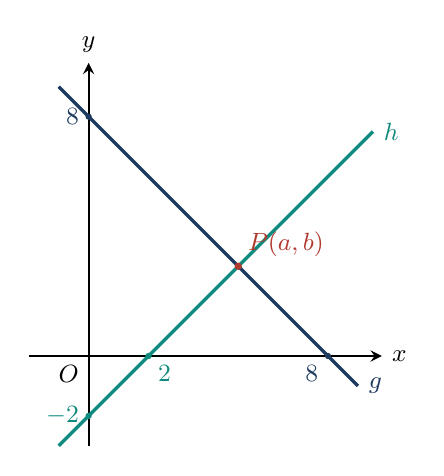
\begin{tikzpicture}[scale=0.38,>=stealth,font=\small]
\draw[->,thick] (-2,0)--(9.8,0) node[right]{$x$};
\draw[->,thick] (0,-3)--(0,9.8) node[above]{$y$};
\draw[navy,very thick] (-1,9)--(9,-1) node[right]{$g$};
\draw[teal,very thick] (-1,-3)--(9.5,7.5) node[right]{$h$};
\fill[navy] (8,0) circle(3pt) node[below left]{$8$};
\fill[navy] (0,8) circle(3pt) node[left]{$8$};
\fill[teal] (2,0) circle(3pt) node[below right]{$2$};
\fill[teal] (0,-2) circle(3pt) node[left]{$-2$};
\fill[brick] (5,3) circle(3.5pt) node[above right]{$P(a,b)$};
\node[below left] at (0,0) {$O$};
\end{tikzpicture}\end{minipage}\vspace{-0.3em}}{\begin{tabularx}{\linewidth}{@{}*{5}{X}@{}}\textbf{A.}\;$12$ & \textbf{B.}\;$15$ & \textbf{C.}\;$16$ & \textbf{D.}\;$18$ & \textbf{E.}\;$20$\end{tabularx}}
\soal{Himpunan penyelesaian pertidaksamaan $4-3x>10$ adalah \dots.}{\begin{tabularx}{\linewidth}{@{}*{5}{X}@{}}\textbf{A.}\;$x<-2$ & \textbf{B.}\;$x>-2$ & \textbf{C.}\;$x<2$ & \textbf{D.}\;$x>2$ & \textbf{E.}\;$x<-6$\end{tabularx}}
\soal{Harga 3 buku dan 2 pensil Rp21.000, sedangkan harga 1 buku dan 2 pensil Rp11.000. Harga 4 buku dan 3 pensil adalah \dots.}{\begin{tabularx}{\linewidth}{@{}*{5}{X}@{}}\textbf{A.}\;Rp24.000 & \textbf{B.}\;Rp26.000 & \textbf{C.}\;Rp27.000 & \textbf{D.}\;Rp29.000 & \textbf{E.}\;Rp31.000\end{tabularx}}
\soal{Himpunan penyelesaian pertidaksamaan $|x-2|<3$ adalah \dots.}{\begin{tabularx}{\linewidth}{@{}*{3}{X}@{}}\textbf{A.}\;$x<-1$ atau $x>5$ & \textbf{B.}\;$x<5$ & \textbf{C.}\;$1<x<5$\\[3pt] \textbf{D.}\;$-5<x<1$ & \textbf{E.}\;$-1<x<5$ & \end{tabularx}}
\soal{Jika $101x+99y=301$ dan $99x+101y=299$, maka nilai $x^{2}-y^{2}$ adalah \dots.}{\begin{tabularx}{\linewidth}{@{}*{5}{X}@{}}\textbf{A.}\;$1$ & \textbf{B.}\;$3$ & \textbf{C.}\;$5$ & \textbf{D.}\;$7$ & \textbf{E.}\;$9$\end{tabularx}}
\soal{Jika $(x,y,z)$ adalah penyelesaian sistem \[\begin{cases}x+y+z=6\\ 2x-y+z=3\\ x+2y-z=2\end{cases}\] maka nilai $x+2y+3z$ adalah \dots.}{\begin{tabularx}{\linewidth}{@{}*{5}{X}@{}}\textbf{A.}\;$10$ & \textbf{B.}\;$11$ & \textbf{C.}\;$12$ & \textbf{D.}\;$13$ & \textbf{E.}\;$14$\end{tabularx}}
\soal{Sistem persamaan $2x+ky=9$ dan $x+3y=4$ tidak mempunyai penyelesaian jika $k=$ \dots.}{\begin{tabularx}{\linewidth}{@{}*{5}{X}@{}}\textbf{A.}\;$2$ & \textbf{B.}\;$3$ & \textbf{C.}\;$6$ & \textbf{D.}\;$9$ & \textbf{E.}\;$12$\end{tabularx}}
\soal{Himpunan penyelesaian pertidaksamaan $\dis\frac{2x-1}{x+2}\le1$ adalah \dots.}{\begin{tabularx}{\linewidth}{@{}*{3}{X}@{}}\textbf{A.}\;$-2<x\le3$ & \textbf{B.}\;$x\le3$ & \textbf{C.}\;$x<-2$ atau $x\ge3$\\[3pt] \textbf{D.}\;$-2\le x\le3$ & \textbf{E.}\;$x\le-2$ atau $x>3$ & \end{tabularx}}
\soal{Jumlah semua bilangan bulat $x$ yang memenuhi $|2x-3|\le5$ adalah \dots.}{\begin{tabularx}{\linewidth}{@{}*{5}{X}@{}}\textbf{A.}\;$4$ & \textbf{B.}\;$6$ & \textbf{C.}\;$7$ & \textbf{D.}\;$9$ & \textbf{E.}\;$10$\end{tabularx}}
\soal{Andi membeli 3 buku, 2 pulpen, dan 1 penggaris seharga Rp22.000. Budi membeli 2 buku, 3 pulpen, dan 2 penggaris seharga Rp21.000. Citra membeli 1 buku, 1 pulpen, dan 3 penggaris seharga Rp11.000. Harga 1 buku, 1 pulpen, dan 1 penggaris seluruhnya adalah \dots.}{\begin{tabularx}{\linewidth}{@{}*{5}{X}@{}}\textbf{A.}\;Rp7.000 & \textbf{B.}\;Rp8.000 & \textbf{C.}\;Rp8.500 & \textbf{D.}\;Rp9.000 & \textbf{E.}\;Rp10.000\end{tabularx}}
\soal{Himpunan penyelesaian pertidaksamaan $|x+1|\ge2|x-2|$ adalah \dots.}{\begin{tabularx}{\linewidth}{@{}*{3}{X}@{}}\textbf{A.}\;$1\le x\le5$ & \textbf{B.}\;$x\le1$ atau $x\ge5$ & \textbf{C.}\;$-1\le x\le2$\\[3pt] \textbf{D.}\;$-5\le x\le-1$ & \textbf{E.}\;$1<x<5$ & \end{tabularx}}
\soal{Diketahui sistem persamaan $2x+y=k+3$ dan $x-y=2k-3$. Penyelesaian $(x,y)$ terletak di kuadran IV jika \dots.}{\begin{tabularx}{\linewidth}{@{}*{5}{X}@{}}\textbf{A.}\;$k<0$ & \textbf{B.}\;$0<k<3$ & \textbf{C.}\;$k>3$ & \textbf{D.}\;$k>0$ & \textbf{E.}\;$k<3$\end{tabularx}}
\soal{Seorang perajin membuat meja dan kursi. Satu meja memerlukan 3 jam perakitan dan 1 jam pengecatan, sedangkan satu kursi memerlukan 2 jam perakitan dan 2 jam pengecatan. Waktu yang tersedia adalah 36 jam perakitan dan 20 jam pengecatan. Keuntungan tiap meja Rp200.000 dan tiap kursi Rp100.000. Keuntungan maksimum yang dapat diperoleh adalah \dots.}{\begin{tabularx}{\linewidth}{@{}*{3}{X}@{}}\textbf{A.}\;Rp1.800.000 & \textbf{B.}\;Rp2.000.000 & \textbf{C.}\;Rp2.200.000\\[3pt] \textbf{D.}\;Rp2.300.000 & \textbf{E.}\;Rp2.400.000 & \end{tabularx}}
\soal{\begin{minipage}[t]{0.55\linewidth}Daerah yang diarsir pada gambar berikut merupakan himpunan penyelesaian suatu sistem pertidaksamaan linear. Luas daerah arsiran adalah \dots\ satuan luas.\end{minipage}\hfill\begin{minipage}[t]{0.43\linewidth}\vspace{0pt}\centering 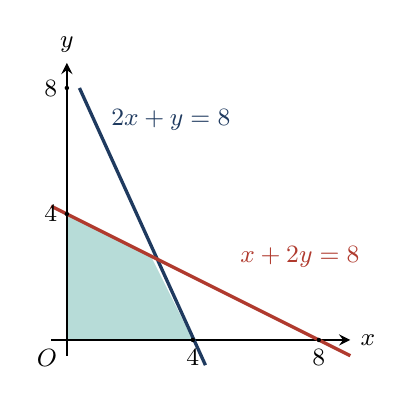
\begin{tikzpicture}[scale=0.40,>=stealth,font=\small]
\fill[teal!30] (0,0)--(4,0)--(8/3,8/3)--(0,4)--cycle;
\draw[->,thick] (-0.5,0)--(9,0) node[right]{$x$};
\draw[->,thick] (0,-0.5)--(0,8.8) node[above]{$y$};
\draw[navy,very thick] (4.4,-0.8)--(0.4,8) ;
\draw[brick,very thick] (9,-0.5)--(-0.5,4.25);
\node[navy,right] at (1.1,7) {$2x+y=8$};
\node[brick,above right] at (5.2,2) {$x+2y=8$};
\foreach \p/\l in {(4,0)/4,(8,0)/8} \fill \p circle(2pt) node[below]{$\l$};
\foreach \p/\l in {(0,4)/4,(0,8)/8} \fill \p circle(2pt) node[left]{$\l$};
\node[below left] at (0,0) {$O$};
\end{tikzpicture}\end{minipage}\vspace{-0.3em}}{\begin{tabularx}{\linewidth}{@{}*{5}{X}@{}}\textbf{A.}\;$8$ & \textbf{B.}\;$\dis\frac{32}{3}$ & \textbf{C.}\;$12$ & \textbf{D.}\;$14$ & \textbf{E.}\;$16$\end{tabularx}}
\soal{Diberikan sistem $ax+y=2$ dan $x+ay=2$ dengan $a$ bilangan real. Perhatikan pernyataan berikut.\par\smallskip\hspace*{0.3em}(1) Jika $a=1$, sistem memiliki tak hingga banyak penyelesaian.\par\hspace*{0.3em}(2) Jika $a=-1$, sistem tidak memiliki penyelesaian.\par\hspace*{0.3em}(3) Jika $a\neq\pm1$, penyelesaian sistem selalu memenuhi $x=y$.\par\hspace*{0.3em}(4) Jika $a=2$, penyelesaian sistem adalah $(1,1)$.\par\smallskip Pernyataan yang benar adalah \dots.}{\begin{tabularx}{\linewidth}{@{}*{3}{X}@{}}\textbf{A.}\;(4) saja & \textbf{B.}\;(1) dan (2) saja & \textbf{C.}\;(2) dan (4) saja\\[3pt] \textbf{D.}\;(1) dan (3) saja & \textbf{E.}\;(1), (2), dan (3) & \end{tabularx}}
\soal{Sebuah toko membuat paket hadiah. Paket jenis A berisi 3 cokelat dan paket jenis B berisi 5 cokelat. Seluruhnya dipakai tepat 115 cokelat, setiap jenis dibuat paling sedikit satu paket, dan banyak paket A lebih banyak daripada paket B. Banyak kemungkinan pasangan (banyak paket A, banyak paket B) adalah \dots.}{\begin{tabularx}{\linewidth}{@{}*{5}{X}@{}}\textbf{A.}\;$3$ & \textbf{B.}\;$4$ & \textbf{C.}\;$5$ & \textbf{D.}\;$6$ & \textbf{E.}\;$7$\end{tabularx}}
\soal{\begin{minipage}[t]{0.55\linewidth}Daerah yang diarsir pada gambar berikut adalah himpunan penyelesaian suatu sistem pertidaksamaan. Sistem pertidaksamaan tersebut adalah \dots.\end{minipage}\hfill\begin{minipage}[t]{0.43\linewidth}\vspace{0pt}\centering 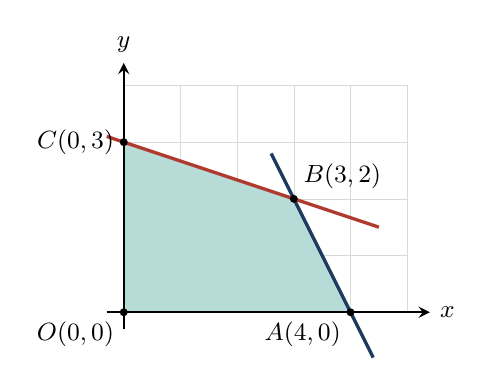
\begin{tikzpicture}[scale=0.72,>=stealth,font=\small]
\draw[gray!30,very thin] (0,0) grid (5,4);
\fill[teal!30] (0,0)--(4,0)--(3,2)--(0,3)--cycle;
\draw[->,thick] (-0.3,0)--(5.4,0) node[right]{$x$};
\draw[->,thick] (0,-0.3)--(0,4.4) node[above]{$y$};
\draw[navy,very thick] (4.4,-0.8)--(2.6,2.8);
\draw[brick,very thick] (-0.3,3.1)--(4.5,1.5);
\fill (0,0) circle(2pt) node[below left]{$O(0,0)$};
\fill (4,0) circle(2pt) node[below left]{$A(4,0)$};
\fill (3,2) circle(2pt) node[above right]{$B(3,2)$};
\fill (0,3) circle(2pt) node[left]{$C(0,3)$};
\end{tikzpicture}\end{minipage}\vspace{-0.3em}}{\begin{tabularx}{\linewidth}{@{}X@{}}\textbf{A.}\;$x\ge0,\ y\ge0,\ x+2y\le8,\ 3x+y\le9$\\ \textbf{B.}\;$x\ge0,\ y\ge0,\ 2x+y\le8,\ x+3y\le9$\\ \textbf{C.}\;$x\ge0,\ y\ge0,\ 2x+y\le8,\ x+3y\ge9$\\ \textbf{D.}\;$x\ge0,\ y\ge0,\ 2x+y\ge8,\ x+3y\le9$\\ \textbf{E.}\;$x\ge0,\ y\ge0,\ 2x+y\le9,\ x+3y\le8$\end{tabularx}}
\soal{Diketahui daerah penyelesaian sistem $x\ge0$, $y\ge0$, $2x+y\le8$, dan $x+3y\le9$. Fungsi $Z=ax+y$ dengan $a>0$ mencapai nilai maksimum di lebih dari satu titik pada daerah tersebut. Nilai $a$ yang mungkin adalah \dots.}{\begin{tabularx}{\linewidth}{@{}*{3}{X}@{}}\textbf{A.}\;$\dis\frac13$ atau $2$ & \textbf{B.}\;$\dis\frac12$ atau $3$ & \textbf{C.}\;$\dis\frac13$ saja\\[3pt] \textbf{D.}\;$2$ saja & \textbf{E.}\;$\dis\frac13$, $1$, atau $2$ & \end{tabularx}}
\soal{Pada sebuah ujian terdapat 30 soal. Jawaban benar diberi skor $4$, jawaban salah diberi skor $-1$, dan soal tidak dijawab diberi skor $0$. Budi memperoleh skor $70$. Banyak soal yang dijawab Budi dengan benar paling sedikit dan paling banyak berturut-turut adalah \dots.}{\begin{tabularx}{\linewidth}{@{}*{3}{X}@{}}\textbf{A.}\;$17$ dan $20$ & \textbf{B.}\;$18$ dan $19$ & \textbf{C.}\;$19$ dan $20$\\[3pt] \textbf{D.}\;$18$ dan $20$ & \textbf{E.}\;$17$ dan $19$ & \end{tabularx}}
\bagian{B. Isian Singkat}{5 soal $\times$ 4 poin = 20 poin. Tuliskan hanya jawaban akhir.}
\soal{Banyak bilangan bulat $x$ yang memenuhi $\dis\frac{3-x}{x+4}\ge0$ adalah \dots}{\jwb}
\soal{Garis $(a+1)x+(2a-1)y=15$ melalui titik potong garis $x+2y=7$ dan garis $3x-y=7$. Nilai $a$ adalah \dots}{\jwb}
\soal{Jika $x$ dan $y$ memenuhi $\dis\frac{3}{x+1}+\dis\frac{2}{y-2}=\dis\frac53$ dan $\dis\frac{6}{x+1}-\dis\frac{3}{y-2}=1$, maka nilai $x+y$ adalah \dots}{\jwb}
\soal{Diketahui bilangan real $x,y,z$ dengan $x+y+z=27$ dan $\dis\frac{x+y}{2}=\dfrac{y+z}{3}=\dfrac{z+x}{4}$. Nilai $xyz$ adalah \dots}{\jwb}
\soal{Seorang petani memerlukan paling sedikit $12$ unit nitrogen dan $20$ unit fosfor. Satu kantong pupuk P mengandung $1$ unit nitrogen dan $3$ unit fosfor dengan harga Rp3.000, sedangkan satu kantong pupuk Q mengandung $2$ unit nitrogen dan $2$ unit fosfor dengan harga Rp2.500. Biaya minimum pembelian pupuk adalah Rp \dots}{\jwb}
\bagian{C. Uraian (Essay)}{5 soal $\times$ 8 poin = 40 poin. Tuliskan langkah penyelesaian dengan lengkap.}
\soal{Pada hari Senin, Ani membeli 5 kg jeruk dan 3 kg apel seharga Rp145.000. Pada hari Selasa, ia membeli 3 kg jeruk dan 4 kg apel seharga Rp120.000.\par\smallskip\hspace*{0.3em}(a) Susun model matematika berupa sistem persamaan linear dua variabel.\par\hspace*{0.3em}(b) Tentukan harga 1 kg jeruk dan 1 kg apel dengan metode eliminasi.\par\hspace*{0.3em}(c) Jika Ani membeli 7 kg jeruk dan 6 kg apel lalu membayar dengan uang Rp250.000, berapa uang kembaliannya?}{\poin{8}}
\soal{Tentukan himpunan penyelesaian dari\par\smallskip\hspace*{0.3em}(a) $\dis\frac{x+1}{x-2}\ge2$,\par\hspace*{0.3em}(b) $|2x-3|\ge3$,\par\hspace*{0.3em}(c) kedua pertidaksamaan pada (a) dan (b) berlaku sekaligus.}{\poin{8}}
\soal{Diketahui sistem persamaan $x+ay=2$ dan $ax+4y=4$.\par\smallskip\hspace*{0.3em}(a) Tentukan nilai $a$ agar sistem memiliki tak hingga banyak penyelesaian dan nilai $a$ agar sistem tidak memiliki penyelesaian. Jelaskan alasannya.\par\hspace*{0.3em}(b) Untuk $a\neq\pm2$, nyatakan $x$ dan $y$ dalam $a$.\par\hspace*{0.3em}(c) Tentukan semua bilangan bulat $a$ sehingga $x$ dan $y$ keduanya bilangan bulat.}{\poin{8}}
\soal{Sebuah toko kue membuat dua jenis kue. Satu kue A memerlukan 200 gram tepung dan 100 gram mentega, sedangkan satu kue B memerlukan 100 gram tepung dan 300 gram mentega. Persediaan yang ada adalah 4 kg tepung dan 4,5 kg mentega. Keuntungan tiap kue A Rp5.000 dan tiap kue B Rp4.000.\par\smallskip\hspace*{0.3em}(a) Susun model matematikanya (sistem pertidaksamaan dan fungsi tujuan).\par\hspace*{0.3em}(b) Tentukan titik-titik sudut daerah penyelesaiannya.\par\hspace*{0.3em}(c) Tentukan banyak kue A dan kue B agar keuntungan maksimum, beserta keuntungan maksimumnya.}{\poin{8}}
\soal{Seorang apoteker mencampur tiga larutan asam, yaitu A (kadar $20\%$), B (kadar $50\%$), dan C (kadar $80\%$), untuk memperoleh $60$ liter larutan berkadar $60\%$. Banyak larutan C yang dipakai tiga kali banyak larutan A.\par\smallskip\hspace*{0.3em}(a) Susun sistem persamaan linear tiga variabel dari keterangan tersebut.\par\hspace*{0.3em}(b) Tentukan volume masing-masing larutan.\par\hspace*{0.3em}(c) Dengan syarat volume total $60$ liter dan C tiga kali A, apakah mungkin diperoleh larutan berkadar $75\%$? Jelaskan.}{\poin{8}}
\newpage
\bagian{Kunci Jawaban dan Pembahasan Singkat}{Untuk guru dan pembahasan mandiri}
\par\vspace{0.6em}{\bfseries\color{navy}Kunci Pilihan Ganda}\par\vspace{0.3em}
\begin{tabularx}{\linewidth}{@{}*{10}{>{\centering\arraybackslash}X}@{}}\hline \textbf{1} & \textbf{2} & \textbf{3} & \textbf{4} & \textbf{5} & \textbf{6} & \textbf{7} & \textbf{8} & \textbf{9} & \textbf{10}\\ \hline C & B & A & D & E & B & E & C & A & D\\ \hline\end{tabularx}\par\vspace{0.4em}\begin{tabularx}{\linewidth}{@{}*{10}{>{\centering\arraybackslash}X}@{}}\hline \textbf{11} & \textbf{12} & \textbf{13} & \textbf{14} & \textbf{15} & \textbf{16} & \textbf{17} & \textbf{18} & \textbf{19} & \textbf{20}\\ \hline D & A & C & E & B & E & C & B & A & D\\ \hline\end{tabularx}
\par\vspace{0.8em}{\bfseries\color{navy}Pembahasan Pilihan Ganda}\par\vspace{0.2em}
\small\begin{enumerate}[leftmargin=2em,itemsep=2pt,topsep=2pt]
\item[\textbf{1.}] \textbf{(C)} $2x-6+5=3x-4\Rightarrow 2x-1=3x-4\Rightarrow x=3$.
\item[\textbf{2.}] \textbf{(B)} Jumlahkan: $2x=10\Rightarrow x=5$, sehingga $y=3$. Maka $xy=15$.
\item[\textbf{3.}] \textbf{(A)} $-3x>6$. Dibagi $-3$, tanda berbalik: $x<-2$.
\item[\textbf{4.}] \textbf{(D)} Kurangkan kedua persamaan: 2 buku $=$ Rp10.000, jadi buku Rp5.000. Lalu $2$ pensil $=11.000-5.000=6.000$, jadi pensil Rp3.000. Maka $4(5.000)+3(3.000)=29.000$.
\item[\textbf{5.}] \textbf{(E)} $|x-2|<3\Rightarrow-3<x-2<3\Rightarrow-1<x<5$.
\item[\textbf{6.}] \textbf{(B)} Jumlahkan: $200(x+y)=600\Rightarrow x+y=3$. Kurangkan: $2(x-y)=2\Rightarrow x-y=1$. Maka $x^{2}-y^{2}=(x+y)(x-y)=3$.
\item[\textbf{7.}] \textbf{(E)} Jumlahkan persamaan ke-2 dan ke-3: $3x+y=5$. Jumlahkan persamaan ke-1 dan ke-3: $2x+3y=8$. Dari $y=5-3x$ diperoleh $2x+15-9x=8\Rightarrow x=1$, $y=2$, $z=3$. Maka $x+2y+3z=1+4+9=14$.
\item[\textbf{8.}] \textbf{(C)} Tanpa penyelesaian bila koefisien sebanding tetapi konstanta tidak: $\dis\frac21=\dfrac k3\neq\dfrac94\Rightarrow k=6$ (dan $2\neq\frac94$, jadi memenuhi).
\item[\textbf{9.}] \textbf{(A)} $\dis\frac{2x-1}{x+2}-1\le0\Rightarrow\dfrac{x-3}{x+2}\le0$. Pembuat nol: $x=3$ (ikut) dan $x=-2$ (tidak ikut, penyebut nol). Maka $-2<x\le3$.
\item[\textbf{10.}] \textbf{(D)} $-5\le2x-3\le5\Rightarrow-1\le x\le4$. Bilangan bulatnya $-1,0,1,2,3,4$ dengan jumlah $9$.
\item[\textbf{11.}] \textbf{(D)} Jumlahkan ketiga persamaan: $6(\text{buku}+\text{pulpen}+\text{penggaris})=22.000+21.000+11.000=54.000$. Maka harga ketiganya Rp9.000. (Cek: buku 5.000, pulpen 3.000, penggaris 1.000.)
\item[\textbf{12.}] \textbf{(A)} Kedua ruas tak negatif, jadi boleh dikuadratkan: $(x+1)^{2}\ge4(x-2)^{2}\Rightarrow3x^{2}-18x+15\le0\Rightarrow(x-1)(x-5)\le0$. Maka $1\le x\le5$.
\item[\textbf{13.}] \textbf{(C)} Jumlahkan kedua persamaan: $3x=3k\Rightarrow x=k$, sehingga $y=3-k$. Kuadran IV: $x>0$ dan $y<0$, yaitu $k>0$ dan $k>3$. Irisannya $k>3$.
\item[\textbf{14.}] \textbf{(E)} Misal $x$ meja, $y$ kursi: $3x+2y\le36$, $x+2y\le20$, $x,y\ge0$, $Z=200.000x+100.000y$. Titik sudut: $(0,0)$, $(12,0)$, $(8,6)$, $(0,10)$ dengan $Z=0$; $2.400.000$; $2.200.000$; $1.000.000$. Maksimum Rp2.400.000 (bukan di titik potong kedua garis).
\item[\textbf{15.}] \textbf{(B)} Titik sudut: $(0,0)$, $(4,0)$, $\left(\frac83,\frac83\right)$, $(0,4)$ (titik potong dari $2x+y=8$ dan $x+2y=8$). Daerah dibagi dua segitiga: $\frac12\cdot4\cdot\frac83+\frac12\cdot4\cdot\frac83=\dis\frac{32}{3}$.
\item[\textbf{16.}] \textbf{(E)} Kurangkan kedua persamaan: $(a-1)(x-y)=0$. (1) $a=1$: kedua persamaan sama ($x+y=2$), tak hingga penyelesaian, \emph{benar}. (2) $a=-1$: $-x+y=2$ dan $x-y=2$ bertentangan, \emph{benar}. (3) $a\neq1\Rightarrow x=y$, \emph{benar}. (4) $a=2$: $x=y=\frac23\neq1$, \emph{salah}.
\item[\textbf{17.}] \textbf{(C)} $3a+5b=115$ dengan $a>b\ge1$. Agar $a=\frac{115-5b}{3}$ bulat, $b\equiv2\pmod3$, yaitu $b=2,5,8,11,14,\dots$ dengan $a=35,30,25,20,15,\dots$. Syarat $a>b$ dipenuhi untuk $b=2,5,8,11,14$ (untuk $b=17$, $a=10<17$). Ada $5$ pasangan.
\item[\textbf{18.}] \textbf{(B)} Garis $AB$ melalui $(4,0)$ dan $(3,2)$: $2x+y=8$. Garis $BC$ melalui $(3,2)$ dan $(0,3)$: $x+3y=9$. Titik $O(0,0)$ ada di daerah dan memenuhi $0\le8$ serta $0\le9$, sehingga tanda $\le$. Ditambah $x\ge0$, $y\ge0$.
\item[\textbf{19.}] \textbf{(A)} Nilai $Z$ di titik sudut: $O:0$; $A(4,0):4a$; $B(3,2):3a+2$; $C(0,3):3$. Maksimum di lebih dari satu titik bila garis selidik sejajar sisi $AB$ atau $BC$. Sejajar $AB$ ($2x+y=8$): $a=2$, nilai $8$ di $A$ dan $B$. Sejajar $BC$ ($\frac13x+y=3$): $a=\frac13$, nilai $3$ di $B$ dan $C$. Untuk $a$ lain, maksimum hanya di satu titik.
\item[\textbf{20.}] \textbf{(D)} Misal benar $b$, salah $s$, kosong $k$: $b+s+k=30$ dan $4b-s=70$. Maka $s=4b-70\ge0\Rightarrow b\ge18$ (karena $b$ bulat), dan $k=100-5b\ge0\Rightarrow b\le20$. Jadi $b\in\{18,19,20\}$: paling sedikit $18$, paling banyak $20$.
\end{enumerate}
\par\Needspace{6\baselineskip}\vspace{0.6em}{\bfseries\color{navy}\normalsize Pembahasan Isian Singkat}\par\vspace{0.2em}
\small\begin{enumerate}[leftmargin=2em,itemsep=2pt,topsep=2pt]
\item[\textbf{1.}] \textbf{Jawaban: $7$.} Pembuat nol: $x=3$ (ikut) dan $x=-4$ (tidak ikut). Penyelesaiannya $-4<x\le3$, yaitu bilangan bulat $-3,-2,\dots,3$ sebanyak $7$.
\item[\textbf{2.}] \textbf{Jawaban: $2$.} Titik potong: dari $x+2y=7$ dan $3x-y=7$ diperoleh $x=3$, $y=2$. Substitusi: $3(a+1)+2(2a-1)=15\Rightarrow7a+1=15\Rightarrow a=2$.
\item[\textbf{3.}] \textbf{Jawaban: $7$.} Misal $u=\frac1{x+1}$, $v=\frac1{y-2}$: $3u+2v=\frac53$ dan $6u-3v=1$. Dua kali persamaan pertama dikurangi persamaan kedua: $7v=\frac73\Rightarrow v=\frac13$, lalu $u=\frac13$. Jadi $x+1=3$, $y-2=3$, sehingga $x=2$, $y=5$, dan $x+y=7$.
\item[\textbf{4.}] \textbf{Jawaban: $405$.} Misal $x+y=2t$, $y+z=3t$, $z+x=4t$. Jumlahnya: $2(x+y+z)=9t\Rightarrow t=6$. Maka $x+y=12$, $y+z=18$, $z+x=24$, sehingga $z=27-12=15$, $x=27-18=9$, $y=27-24=3$. $xyz=405$.
\item[\textbf{5.}] \textbf{Jawaban: $22.000$.} Model: $x+2y\ge12$, $3x+2y\ge20$, $x,y\ge0$, minimumkan $Z=3000x+2500y$. Titik sudut: $(0,10)$, $(12,0)$, $(4,4)$ dengan $Z=25.000$; $36.000$; $22.000$. Minimum Rp22.000.
\end{enumerate}
\par\Needspace{8\baselineskip}\vspace{0.6em}{\bfseries\color{navy}\normalsize Pembahasan dan Pedoman Penskoran Uraian}\par\vspace{0.2em}
\small\begin{enumerate}[leftmargin=2em,itemsep=3pt,topsep=2pt]
\item[\textbf{1.}] (a) Misal $x$ harga 1 kg jeruk dan $y$ harga 1 kg apel: $5x+3y=145.000$ dan $3x+4y=120.000$. (b) Kalikan 3 dan 5: $15x+9y=435.000$ dan $15x+20y=600.000$. Kurangkan: $11y=165.000\Rightarrow y=15.000$. Maka $x=\frac{145.000-45.000}{5}=20.000$. Jeruk Rp20.000/kg dan apel Rp15.000/kg. (c) $7(20.000)+6(15.000)=230.000$, kembalian $250.000-230.000=$ Rp20.000. \\ \textit{Penskoran: Model (2 poin); eliminasi dan kedua harga (4 poin); kembalian (2 poin).}
\item[\textbf{2.}] (a) $\dis\frac{x+1}{x-2}-2\ge0\Rightarrow\dfrac{5-x}{x-2}\ge0$. Pembuat nol $x=5$ (ikut) dan $x=2$ (tidak ikut), sehingga $2<x\le5$. (b) $2x-3\ge3$ atau $2x-3\le-3$, yaitu $x\ge3$ atau $x\le0$. (c) Irisan $2<x\le5$ dengan ($x\le0$ atau $x\ge3$) adalah $3\le x\le5$. HP $=\{x\mid3\le x\le5\}$. \\ \textit{Penskoran: Bagian (a) 3 poin; (b) 3 poin; (c) 2 poin.}
\item[\textbf{3.}] (a) Syarat sebanding: $\dis\frac1a=\dfrac a4\Rightarrow a^{2}=4\Rightarrow a=\pm2$. Untuk $a=2$: $x+2y=2$ dan $2x+4y=4$ (persamaan kedua $=2\times$ pertama), jadi tak hingga penyelesaian. Untuk $a=-2$: $x-2y=2$ dan $x-2y=-2$ bertentangan, jadi tidak ada penyelesaian. (b) Kalikan persamaan pertama dengan $a$ lalu kurangkan dari persamaan kedua: $(4-a^{2})y=4-2a\Rightarrow y=\dis\frac{2}{a+2}$. Maka $x=2-ay=\dis\frac{4}{a+2}$. (c) $x,y$ bulat $\Rightarrow(a+2)$ membagi $2$ dan $4$, sehingga $a+2\in\{-2,-1,1,2\}$ dan $a\in\{-4,-3,-1,0\}$ (tidak ada yang sama dengan $\pm2$). \\ \textit{Penskoran: Bagian (a) 3 poin; (b) 3 poin; (c) 2 poin.}
\Needspace{14\baselineskip}\item[\textbf{4.}] (a) Misal $x$ kue A, $y$ kue B: $200x+100y\le4000\Rightarrow2x+y\le40$; $100x+300y\le4500\Rightarrow x+3y\le45$; $x,y\ge0$ (bilangan cacah); maksimumkan $Z=5000x+4000y$. (b) Titik sudut: $(0,0)$, $(20,0)$, $(0,15)$, dan perpotongan kedua garis: $y=40-2x\Rightarrow x+120-6x=45\Rightarrow x=15$, $y=10$, yaitu $(15,10)$. (c) $Z=0$; $100.000$; $60.000$; $115.000$. Untung maksimum Rp115.000 dengan $15$ kue A dan $10$ kue B. \\ \textit{Penskoran: Model (3 poin); titik sudut (3 poin); nilai maksimum dan banyak kue (2 poin).}
\par\vspace{0.3em}\begin{center}
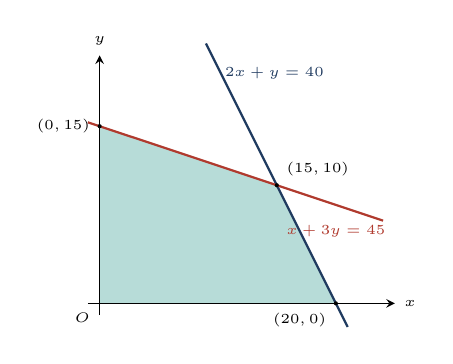
\begin{tikzpicture}[scale=0.15,>=stealth,font=\tiny]
\fill[teal!30] (0,0)--(20,0)--(15,10)--(0,15)--cycle;
\draw[->] (-1,0)--(25,0) node[right]{$x$};
\draw[->] (0,-1)--(0,21) node[above]{$y$};
\draw[navy,thick] (21,-2)--(9,22);
\draw[brick,thick] (-1,15.33)--(24,7);
\node[navy,right] at (9.8,19.5) {$2x+y=40$};
\node[brick,below] at (20,7.4) {$x+3y=45$};
\fill (20,0) circle(5pt) node[below left]{$(20,0)$};
\fill (15,10) circle(5pt) node[above right]{$(15,10)$};
\fill (0,15) circle(5pt) node[left]{$(0,15)$};
\node[below left] at (0,0) {$O$};
\end{tikzpicture}
\end{center}\vspace{-0.4em}
\item[\textbf{5.}] (a) Misal volume A, B, C berturut-turut $x,y,z$ liter: $x+y+z=60$; $0{,}2x+0{,}5y+0{,}8z=0{,}6\cdot60=36$; $z=3x$. (b) Dari $z=3x$: $y=60-4x$. Substitusi ke persamaan kedua (kali 10): $2x+5(60-4x)+24x=360\Rightarrow6x=60\Rightarrow x=10$. Jadi $A=10$ L, $B=20$ L, $C=30$ L. (c) Dengan $z=3x$ dan total $60$ L, banyak asam $=0{,}6x+30$. Karena $y=60-4x\ge0$, maka $0\le x\le15$ sehingga asam berkisar $30$ sampai $39$ liter, yaitu kadar $50\%$ sampai $65\%$. Kadar $75\%$ perlu $x=25$ dan $y=-40<0$, tidak mungkin. \\ \textit{Penskoran: Sistem persamaan (3 poin); volume tiap larutan (3 poin); kesimpulan dengan alasan (2 poin).}
\end{enumerate}
\end{document}
